% para agregar la carpeta de las imagenes
%\graphicspath{{./nombre de la carpeta/}}

%el codigo principal solo contiene el tipo de documento, la caratula y la forma de llamar a los otros archivos, asi como imprimir bibilografia y el indice.

\documentclass[11pt,a4paper]{article}
% Configuración de la codificación de entrada
\usepackage[utf8]{inputenc}

% Configuración de la codificación de salida
\usepackage[T1]{fontenc}

% Paquete para el idioma y comillas
\usepackage[spanish,es-tabla]{babel}
\usepackage{csquotes}

\usepackage{hyphenat}
\usepackage{microtype}

\hyphenation{ex-am-ple hy-phen-a-tion}
\hyphenpenalty=500
\tolerance=1000

% Tamaño de la página (A4) y márgenes
\usepackage[a4paper,top=2cm,bottom=2cm,left=3cm,right=3cm,marginparwidth=1.75cm]{geometry}

% Otros packages
\usepackage{fancyhdr}
\pagestyle{fancy}
\usepackage{amsmath}
\usepackage{graphicx}
\usepackage[colorlinks=true, allcolors=black]{hyperref}
\usepackage[utf8]{inputenc}

\usepackage{hyperref}
\usepackage{amsmath}
\usepackage[usenames]{color}
\usepackage{amsfonts}
\usepackage{amssymb}
\usepackage{graphicx}
\usepackage{caption}
\usepackage{enumerate} 
\usepackage{siunitx}
\usepackage{upgreek}
\usepackage{epsfig}
\usepackage{multirow}
\usepackage{colortbl}
\usepackage{xspace}    

% para las tablas
\usepackage{multicol,multirow, array} 
\usepackage[table,xcdraw]{xcolor}
\usepackage[table]{xcolor}
\captionsetup{justification=centerlast,labelfont=bf,font=sf}
\usepackage{subfigure}
\usepackage[T1]{fontenc}
\usepackage{fourier}
\usepackage{float} 
\usepackage{steinmetz}
\setcounter{equation}{0}
\usepackage{biblatex} %llama al archivo donde estan todas las librerias include


%%encabezado
\rhead{\begin{picture}(0,0)	\put(-15,0) {
\includegraphics[height=1cm]{caratula/logounsl.png}} \end{picture}}
\lhead{\begin{picture}(0,0)	\put(-15,0) {
\includegraphics[height=1cm]{caratula/logo_depto.jpg}} \end{picture}}
\chead{\vspace{-.05cm}\textcolor{gray}{Sistemas de Comunicaciones, teoría de la información y Análisis de Señales - TP N.$^o$3} \vspace{.25cm}}

%%
%pie de pagina
\rfoot{\textcolor{gray}{Comunicaciones I - 2025}}
\lfoot{\textcolor{gray}{Marcos Lucero - Nahuel Ramires - Agustín Cappiello}}
\cfoot{\textcolor{gray}{\thepage}}  % Cambiar el número de página a gris



\begin{document}
    %caratula
    \begin{titlepage}	  
    		\centering
    		
    		% --- Logo UNSL ---		
    		\begin{figure}
    			\centering
    			
\includegraphics[width=0.15\linewidth]{caratula/logo-unsl.jpg}
    		\end{figure}     
    		
    		% --- Datos de la asignatura ---
    		{\scshape\LARGE Universidad Nacional de San Luis\\}
    		{\scshape Facultad de Ciencias Físico Matemáticas y Naturales\par}
    		{\scshape Ingeniería Electrónica con O.S.D.\par}
    		\vspace{2cm} 
    		
    		\Large \textbf {Asignatura:\\} 
    		\bigskip
    		\LARGE {\Huge Comunicaciones I}
    		\vspace{0.3cm}
    		
    		% --- Datos del informe / TP ---
    		\LARGE \textbf {Trabajo Practico N° 3\\} 
    		\vspace{0.7cm}
    		\LARGE \textbf {“Modulación Analógica”}

    		\vspace{2cm}
    		% --- Datos del alumno ---  
    		\LARGE \textbf {Estudiantes:\\} 
    		\LARGE Marcos Lucero \\ Nahuel Ramires\\ Agustín Cappiello\\
    		\bigskip
    		
    		
    		\vspace{1cm}
    		
    		% --- Datos de los profesores ---  
    		\Large \textbf {Profesores Responsables:\\} 
    		\bigskip
    		\Large Alejandro Marwan Geraiges Magrini. \\ Roberto Kiessling.
    		
    		
    		\vspace{3cm}
    		
    		% --- Año ---  
    		\Large \textbf {Año:\\} 
    		\Large 2025	
    	\end{titlepage}
    %fin caratula	
    
    \tableofcontents %Para el indice

%	\chapter {Parte1}
    \section{Ejercicio 1}  
En la Fig.~\ref{fig:1} se puede observar el espectro en frecuencias de la señal de mensaje $m(t)$.  

\begin{figure}[h!]
    \centering
    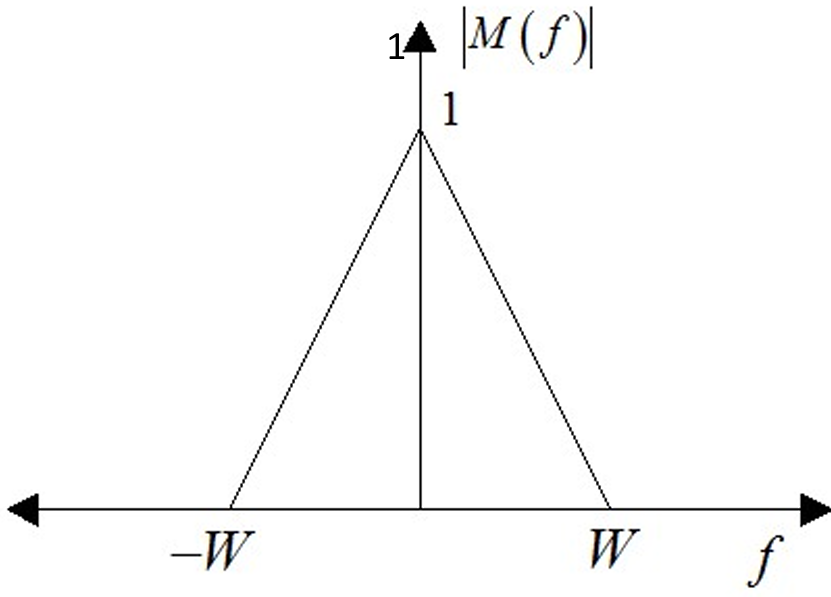
\includegraphics[width=0.6\textwidth]{fig1.png}
    \caption{Espectro de la señal de mensaje $m(t)$}
    \label{fig:1}
\end{figure}

El ancho de banda de la señal es de 1000 Hz, y es aplicada a un modulador producto con portadora $A\cos(2\pi f t)$. La señal modulada $s(t)$ es luego aplicada a un Detector Coherente como el indicado en la Fig.~\ref{fig:2} del Ejercicio 4.  

\begin{itemize}
    \item[a)] Graficar el espectro obtenido en la salida del detector para $f=500$ Hz. ¿Se recibe la señal enviada? Justifique.  
    \item[b)] Repetir para $f=10$ kHz.  
    \item[c)] Determinar la mínima frecuencia de portadora necesaria para recuperar $m(t)$ sin distorsión.  
\end{itemize} %llama los otros 
	\section{Actividad 2}

\subsection*{Un transmisor con modulación de amplitud tiene como entrada una señal $m(t)=A_m\cos(2\pi f t)$ con $A_m=3$ V y $f_m=600$ Hz. 
Si la portadora posee una amplitud de 10 V y una frecuencia de 1 kHz.}  

\subsection*{a)  Calcular de manera analítica la señal de salida del modulador en tiempo y en frecuencia, graficando además los resultados. Suponer un 90\% de porcentaje de modulación. ¿Es posible realizar una detección de envolvente sobre la señal s(t)? o ¿ se requiere una detección coherente?}

En este caso la modulación es de tipo AM (DSB con portadora). La señal portadora modulada de salida se expresa como:

    \[
        s(t) = A_c \left[ 1 + k_a A_m \cos(2\pi f_m t)\right]\cos(2\pi f_c t)
    \]

donde:  

\(A_c\) es la amplitud de la portadora 

\(A_m\) es la amplitud del mensaje

 \(f_c\) es la frecuencia de la portadora
 
 \(f_m\) es la frecuencia de la señal moduladora
 
 \(k_a\) es el la sensibilidad de amplitud del modulador

 \(\mu=k_a A_m\) es el indice de modulación

Al reemplazar los valores dados por el enunciado se obtiene:

    \[
        s(t) = 10\left[1+0.9\cos(2\pi \cdot 600t)\right]\cos(2\pi \cdot 1000t)
    \]
    

Aplicando la propiedad trigonométrica del producto de cosenos:

    \[
        \cos\alpha \cos\beta = \tfrac{1}{2}\left[\cos(\alpha+\beta)+\cos(\alpha-\beta)\right],
    \]

La expresión resultante se desarrolla como:

    \[
        s(t) = A_c\ \cos(2\pi f_c t) \;+\; \frac{A_c \ \mu}{2}\Big[ \cos\big(2\pi(f_c+f_m)t\big) + \cos\big(2\pi(f_c-f_m)t\big) \Big]
    \]


Reemplazando los valores numéricos en la expresión anterior:

    \[
        s(t) = 10\cos(2\pi \cdot 1000 t) \;+\; 4.5 \cos(2\pi \cdot 1600 t) \;+\; 4.5 \cos(2\pi \cdot 400 t)
    \]


\textbf{El desarrollo en frecuencia es el siguiente:}  

La Transformada de Fourier de \(s(t)\) está formada por tres deltas centradas en las frecuencias indicadas:

    \[
        S(f) = \tfrac{A_c}{2}\big[\delta(f-f_c)+\delta(f+f_c)\big] \;+\; 
        \tfrac{A_c \ \mu}{4}\big[\delta(f-(f_c+f_m))+\delta(f+(f_c+f_m))
    \]

    \[
        \;+\;
        \delta(f-(f_c-f_m))+\delta(f+(f_c-f_m))\big]
    \]
Reemplazando por valores numéricos:

    \[
        S(f) = \tfrac{10}{2}\big[\delta(f-1000)+\delta(f+1000)\big] \;+\; 
        \tfrac{9}{4}\big[\delta(f-1600) +\delta(f+1600)
    \]
    \[
        \;+\;
        \delta(f-400)+\delta(f+400)\big]
    \]

Para que la envolvente de la señal s(t) pueda ser detectada la frecuencia de la onda portadora debe cumplir que \(f_c \gg W\). En este caso no se cumple por lo que es necesario un detector coherente para que sea posible.

En la Fig.\ref{fig:actividad_2a} se muestra tanto la señal en el tiempo como su espectro de la señal modulada s(t).

    \begin{figure}[H]
        \centering
        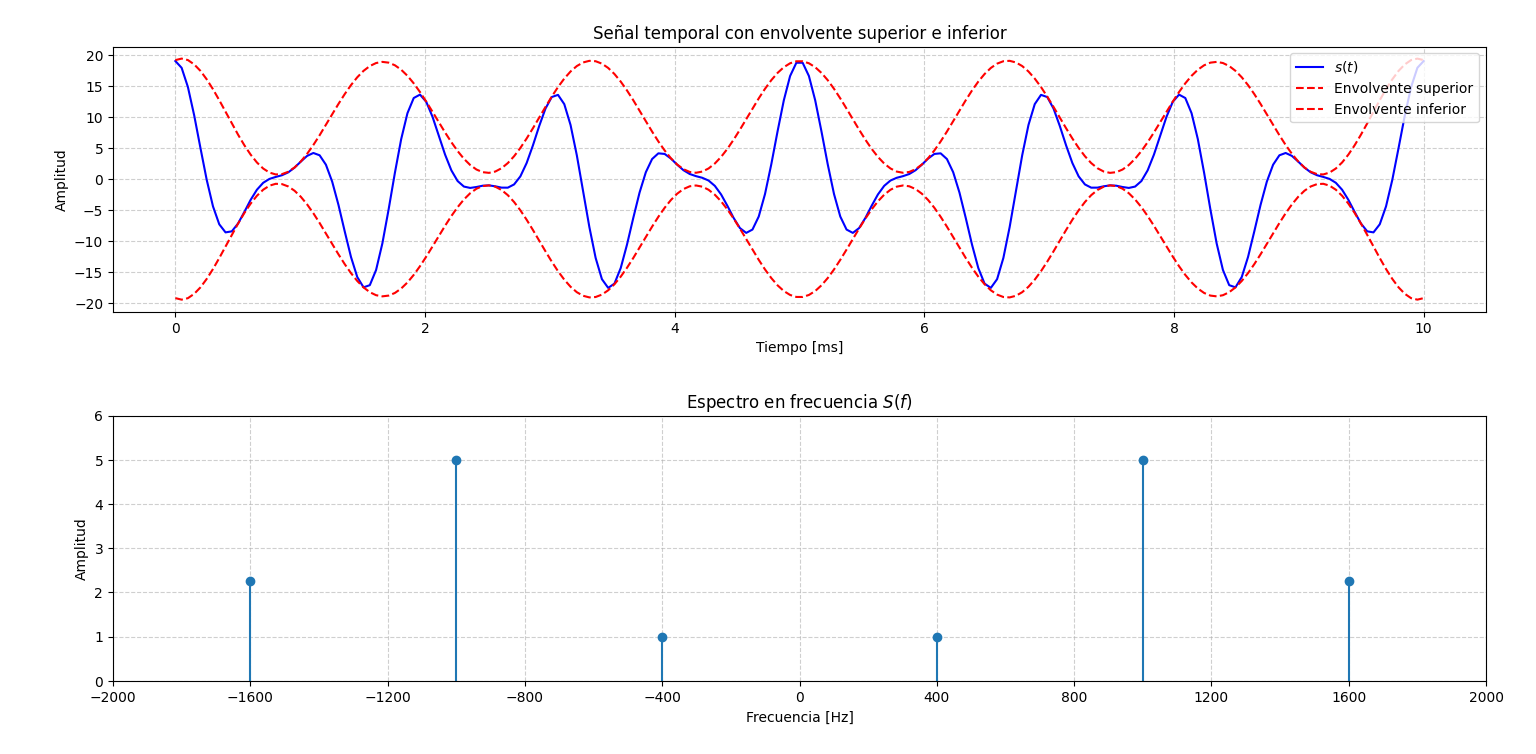
\includegraphics[width=0.9\linewidth]{imagenes/Parte_1/Actividad_2/actividad_2a.png}
        \caption{Señal modulada.}
        \label{fig:actividad_2a}
    \end{figure}

    
\subsection*{b) Modificar la frecuencia de portadora a $f_c=10f_m$ y graficar $s(t)$ para modulaciones 90\% 60\%, 20\% y 110\%. ¿Es posible detección de envolvente en todos los casos? } 

 Expresión analítica para un 90\% de $s(t)$ y $f_c=10 f_m$: 

    \[
        s(t) = 10\left[1+0.9\cos(2\pi \cdot 600t)\right]\cos(2\pi \cdot 6000t)
    \]


 Expresión analítica para un 60\% de $s(t)$ y $f_c=10 f_m$: 

    \[
        s(t) = 10\left[1+0.6\cos(2\pi \cdot 600t)\right]\cos(2\pi \cdot 6000t)
    \]


 Expresión analítica para un 20\% de $s(t)$ y $f_c=10 f_m$: 

    \[
        s(t) = 10\left[1+0.2\cos(2\pi \cdot 600t)\right]\cos(2\pi \cdot 6000t)
    \]

Expresión analítica para un 110\% de $s(t)$ y $f_c=10 f_m$: 

    \[
    s(t) = 10\left[1+1.1\cos(2\pi \cdot 600t)\right]\cos(2\pi \cdot 6000t)
    \]

En la Fig.\ref{fig:actividad_2b} se muestra las gráficas en el dominio del tiempo de la señal $s(t)$ para los distintos factores de modulación $\mu$.

    \begin{figure}[h!]
        \centering
        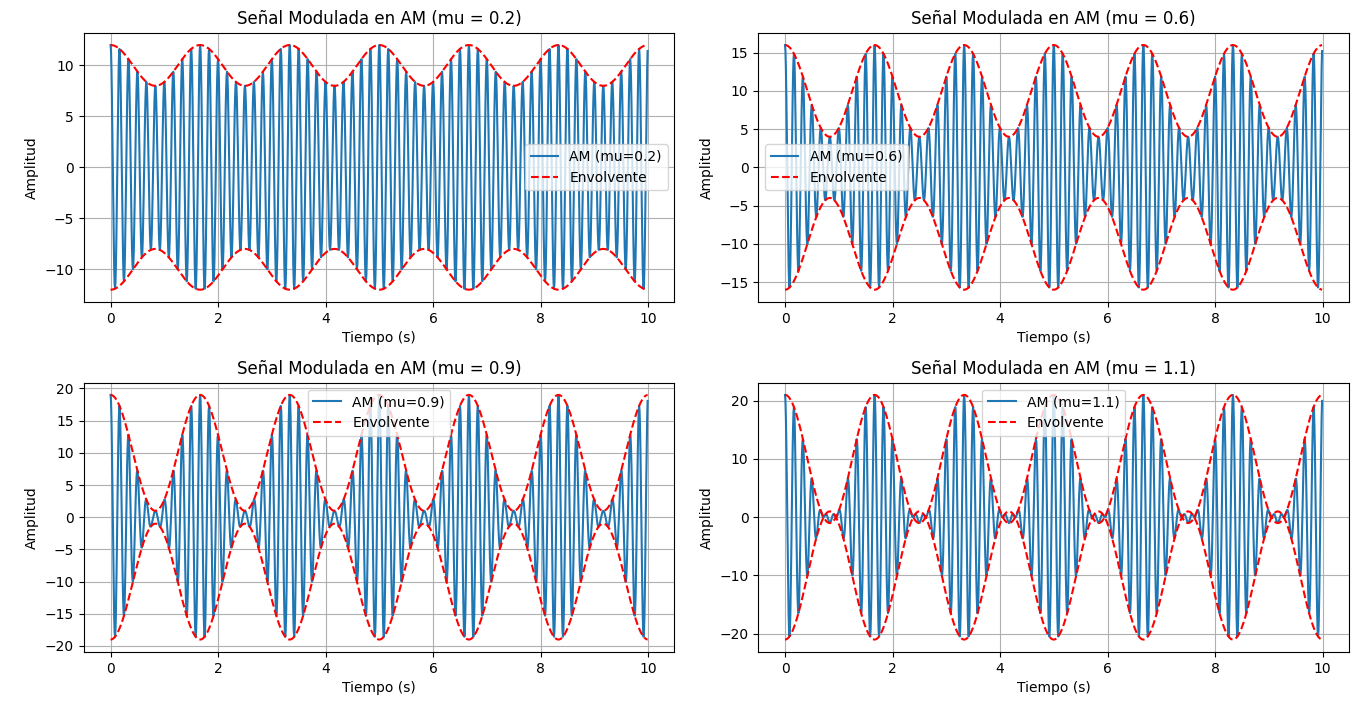
\includegraphics[width=1\textwidth]{imagenes/Parte_1/Actividad_2/actividad_2b.png}
        \caption{Gráfica de $s(t)$ para distintas $\mu$ .}
        \label{fig:actividad_2b}
    \end{figure}

Es posible la detección de envolvente en todos los casos excepto en el porcentaje de 110\% de modulación, ya que cuando la sensibilidad de amplitud $k_a$ del modulador es lo suficientemente grande como para hacer que $|k_a\,m(t)| > 1$ en algún instante de tiempo $t$, la onda portadora se convierte en \textit{sobremodulada}, resultando en una inversión de fase de la onda portadora cuando el factor $(1 + k_a\,m(t))$ cruza por cero. Entonces, la onda modulada exhibe una \textit{distorsión de envolvente}.

Por lo tanto, para evitar la sobremodulación, se debe mantener una relación uno a uno entre la envolvente de la onda AM y la onda modulante, para todos los valores del tiempo.

    


	\section{Actividad 3}

\subsection*{Con los datos del Ejercicio 2, considerar a $s(t)$ una señal de tensión y conectar a la salida del modulador un resistor de $50~\Omega$. Cuando sea posible indicar la respuesta también en dB}.

\subsection*{a) Calcular la potencia media de la portadora para un $\mu = 20\%$.}

La potencia media de portadora para una resistencia de $50~\Omega$ es:
\[
    P_{\text{portadora}} = \frac{1}{2} A_c^2 = \frac{1}{2} \left(10~[V]\right)^2 \frac{1}{50~[\Omega]} = 1~[W]
\]
En dB:
\[
    P_{\text{portadora(dB)}} = 10 \log_{10}(1) = 0~[dBW]
\]

\subsection*{b) Calcular la potencia media de la banda lateral inferior y superior para un $\mu = 20\%$.}

Para una resistencia de $50~\Omega$ las potencias medias de las bandas laterales son:
\[
    P_{BL} = P_{BLS} = \frac{\mu^2 A_c^2}{8R} = \frac{(0.2)^2 (10~[V])^2}{8(50~[\Omega])} = 0.01~[W]
\]
En dB:
\[
    P_{BL(dB)} = 10 \log_{10}(0.01) = -20~[dBW]
\]

\subsection*{c) Calcular la potencia total de las señales moduladas para un $\mu = 20\%$.}

La potencia total es la suma de las tres componentes, potencia media de portadora, de banda superior y banda inferior. El resultado es:
\[
    P_{\text{total}} = P_{\text{portadora}} + P_{BLS} + P_{BLI} = 1.02~[W]
\]
En dB:
\[
    P_{\text{total(dB)}} = 10 \log_{10}(1.02) = 0.087~[dBW]
\]

\subsection*{d) ¿Cuál es la relación de potencia total de banda lateral respecto la potencia total de señal modulada?}

La relación de la potencia total de las bandas laterales con respecto a la potencia total está dada por:
\[
    RP_{\text{bandas}} = \frac{\mu^2}{2 + \mu^2} = \frac{(0.2)^2}{2 + (0.2)^2} = 0.0196 \times 100\% = 1.96\%
\]
En dB:
\[
    RP_{\text{bandas(dB)}} = 10 \log_{10}(0.0196) = -16.9~[dB]
\]

\subsection*{e) ¿Cuál es la relación de potencia total de portadora respecto la potencia total de señal modulada?}

La relación de potencia total de portadora respecto la potencia total de señal modulada se obtiene en base al resultado anterior:
\[
    RP_\textbf{portadora}=\frac{P_\text{portadora}}{P_{\text{total}}} \times 100\% = \frac{1}{1.02} \times 100\% = 98.04\%
\]
En dB:
\[
    RP_{\text{portadora(dB)}} = 10 \log_{10}\left(\frac{1}{1.02}\right) = -0.087~[dB]
\]

\subsection*{f) Repetir nuevamente los cálculos para un $\mu = 100\%$.}

Los cálculos para $\mu = 100\%$ son los siguientes:
\[
    P_{\text{portadora}} = \frac{(10~[V])^2}{2 \cdot 50~[\Omega]} = 1~[W]
\]
En dB:
\[
    P_{\text{portadora(dB)}} = 10 \log_{10}(1) = 0~[dBW]
\]

\[
    P_{BLS} = P_{BLI} = \frac{(10~[V])^2 \cdot 1^2}{8 \cdot 50~[\Omega]} = 0.25~[W]
\]
En dB:
\[
    P_{BL(dB)} = 10 \log_{10}(0.25) = -6.02~[dBW]
\]

\[
    P_{\text{total}} = P_{\text{portadora}} + P_{BLS} + P_{BLI} = 1.5~[W]
\]
En dB:
\[
    P_{\text{total(dB)}} = 10 \log_{10}(1.5) = 1.76~[dBW]
\]

\[
    RP_{\text{bandas}} = \frac{\mu^2}{2 + \mu^2} = \frac{1^2}{2 + 1^2} = \frac{1}{3} \times 100\% = 33.33\%
\]
En dB:
\[
    RP_{\text{bandas(dB)}} = 10 \log_{10}\left(\frac{1}{3}\right) = -4.77~[dB]
\]

\[
    RP_\textbf{portadora}=\frac{P_\text{portadora}}{P_{\text{total}}} \times 100\% = \frac{1}{1.5} \times 100\% = 66.66\%
\]
En dB:
\[
    RP_{\text{portadora(dB)}} = 10 \log_{10}\left(\frac{1}{1.5}\right) = -1.76~[dB]
\]


\subsection*{g) Repasar la teoría y analizar los resultados obtenidos en los puntos anteriores.}

    Al analizar los resultados obtenidos se observa que, para valores bajos del índice de modulación $\mu$, gran parte de la potencia total se concentra en la portadora. Esto no es deseable, ya que aproximadamente el $98{,}04\%$ de la potencia total se gasta en la portadora, la cual no transporta información. 
A medida que el valor de $\mu$ aumenta, la potencia de la portadora permanece constante, pero la proporción de potencia correspondiente a las bandas laterales se incrementa. En consecuencia, una mayor parte de la potencia total se destina a las bandas laterales, que son las que efectivamente contienen la información del mensaje. 

Por lo tanto, se busca trabajar con valores de $\mu$ lo más altos posible sin superar la unidad, para evitar la sobremodulación y la distorsión de la envolvente.

    
\subsection*{h) Comentar las ventajas y desventajas de este tipo de modulación.}

Las ventajas y desventajas de este tipo de modulación, son las siguientes:

\begin{itemize}
    \item Ventajas: La simplicidad que supone a la hora de implementar el receptor.
    \item Desventajas:
        \begin{itemize}
            \item La transmisión de la onda portadora supone una pérdida de potencia para la señal resultante.
            \item La modulación de amplitud malgasta ancho de banda ya que requiere un ancho de banda de transmisión igual al doble del ancho de banda del mensaje.
        \end{itemize}
\end{itemize}
	\section{Ejercicio 4}

Considere la misma señal de mensaje y portadora del Ejercicio 2, pero utilice un modulador producto.

\begin{enumerate}[label=\alph*)]
    \item Expresar analíticamente $s(t)$ y $S(f)$. Graficar resultados y explicar cuál fue el cambio en la señal de salida del modulador.
    \item Considerando que la señal de salida del modulador se aplica a un detector coherente (ver Fig. 2), y que las portadoras tanto en el transmisor como en el receptor se encuentran en perfecto sincronismo: obtener $v(t)$ y graficar su espectro.
    \item Ahora suponer que hay una diferencia de fase entre portadoras. Comentar por qué esto es importante y qué sucede en casos extremos.
\end{enumerate}

\begin{figure}[h!]
    \centering
    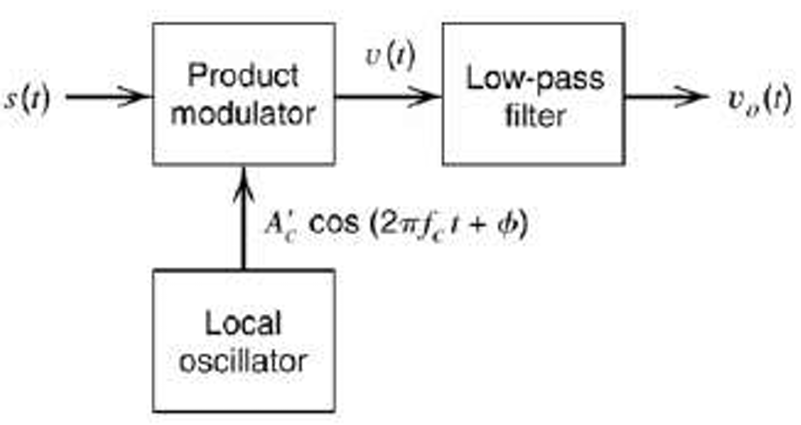
\includegraphics[width=0.7\textwidth]{imagenes/Parte_1/Actividad_4/fig2.png}
    \caption{Detector coherente}
\end{figure}

	\section{Ejercicio 5}

{\subsection*{Una versión particular de AM estéreo usa multiplexación de portadora en cuadratura. Específicamente, la portadora $A_c \cos(2\pi f_c t)$ es empleada para modular la señal suma:}

    \[
        m_1(t) = v_0 + m_l(t) + m_r(t)
    \]

\subsection*{Donde $v_0$ es un \textit{offset DC} incluido con el propósito de transmitir la componente de portadora, 
$m_l(t)$ es la señal de audio del canal izquierdo y $m_r(t)$ es la señal de audio del canal derecho.}

\subsection*{La portadora en cuadratura $A_c \sen(2\pi f_c t)$ es empleada para modular la señal diferencia:}

    \[
        m_2(t) = m_l(t) - m_r(t)
    \]

\subsection*{a) Mostrar que un detector de envolvente puede ser utilizado para recuperar la suma $m_l(t) + m_r(t)$ desde la señal multiplexada en cuadratura. 
¿Cómo puede minimizar la distorsión de la señal producida por el detector de envolvente?}


Un \textbf{detector de envolvente} extrae la envolvente de la señal, que es su amplitud instantánea (magnitud). Para una señal AM estándar, esto recupera el mensaje directamente si hay una portadora fuerte.

Para $s(t)$, la envolvente $E(t)$ es la magnitud de la componente vectorial:
\[ s(t) = I(t) \cos(2\pi f_c t) + Q(t) \sin(2\pi f_c t) \]
donde $I(t) = A_c m_1(t)$ (componente in-fase) y $Q(t) = A_c m_2(t)$ (componente en cuadratura).

La envolvente es:
\[ E(t) = \sqrt{ [A_c m_1(t)]^2 + [A_c m_2(t)]^2 } = A_c \sqrt{ m_1(t)^2 + m_2(t)^2 } \]

Sustituyendo las definiciones:
\[ E(t) = A_c \sqrt{ [v_0 + m_l(t) + m_r(t)]^2 + [m_l(t) - m_r(t)]^2 } \]

Expandimos el cuadrado:
\[ [m_l(t) + m_r(t)]^2 + 2 v_0 [m_l(t) + m_r(t)] + v_0^2 + [m_l(t) - m_r(t)]^2 = 2[m_l(t)^2 + m_r(t)^2] + 2 v_0 [m_l(t) + m_r(t)] + v_0^2 \]
donde los términos cruzados se cancelan.

Si $v_0$ es \textbf{grande} comparado con las amplitudes de $m_l(t)$ y $m_r(t)$ los términos $m_l^2 + m_r^2$ son negligibles. Entonces:
\[ E(t) \approx A_c \sqrt{ v_0^2 + 2 v_0 [m_l(t) + m_r(t)] } = A_c v_0 \sqrt{ 1 + \frac{2 [m_l(t) + m_r(t)]}{v_0} } \]

Usando la aproximación binomial $\sqrt{1 + x} \approx 1 + \frac{x}{2}$ para $x$ pequeño
donde :
\[
x = \frac{2 [m_l(t) + m_r(t)]}{v_0} \ll 1  
\]
Por lo tanto, se obtiene que:
\[ E(t) \approx A_c v_0 \left( 1 + \frac{m_l(t) + m_r(t)}{v_0} \right) = A_c v_0 + A_c [m_l(t) + m_r(t)] \]

Después de filtrar el DC (con un capacitor de acoplamiento), recuperamos $A_c [m_l(t) + m_r(t)]$, que es la suma de los canales (audio mono).

\textbf{Minimización de distorsión}: La distorsión viene de los términos no lineales (como $m_l^2 + m_r^2$) y de la componente en cuadratura $m_d(t)$. Para minimizarla:
    \begin{itemize}
        \item Haz $v_0$ lo suficientemente grande para que el índice de modulación sea bajo (e.g., < 50-70\%), asegurando que la aproximación binomial sea válida y que la envolvente no se distorsione.
        \item Limita la amplitud de $m_d(t)$ (diferencia de canales) para que sea mucho menor que $m_s(t)$.
    \end{itemize}

Esto permite compatibilidad con receptores AM mono, que ignoran la cuadratura y solo oyen la suma.



\subsection*{b) Mostrar que un detector coherente puede recuperar la diferencia $m_l(t) - m_r(t)$.}

Un \textbf{detector coherente} multiplica la señal recibida por una portadora local sincronizada y filtra pasa-bajos. Para recuperar la componente en cuadratura, usamos la portadora desfasada: $2 \sin(2\pi f_c t)$ (el factor 2 es por convención, para simplificar).

Multiplicamos $s(t)$ por $2 \sin(2\pi f_c t)$:
    \[ 
        2 s(t) \sin(2\pi f_c t) = 2 A_c m_1(t) \cos(2\pi f_c t) \sin(2\pi f_c t) + 2 A_c m_2(t) \sin^2(2\pi f_c t)
    \]

Usando identidades trigonométricas:
\begin{itemize}
    \item $2 \cos \theta \sin \theta = \sin(2\theta)$ → término de alta frecuencia (se filtra).
    \item $\sin^2(\theta) = \frac{1 - \cos(2\theta)}{2} \implies 2 \sin^2(\theta) = 1 - \cos(2\theta)$.
\end{itemize}

Se tiene que:
    \[
        Sal(t)= A_c m_1(t) \sin(4\pi f_c t) + A_c m_2(t) \left(1 + \cos(4\pi f_c t)\right)
    \]
    \[
        = A_c m_1(t) \sin(4\pi f_c t) + A_c m_2(t) - A_c m_2(t) \cos(4\pi f_c t)
    \]

Después de filtro pasa-bajos , solo queda el término banda-base de la cuadratura:
\[ 
    Sal_{PB} (t) = A_c m_d(t) \cdot 1 = A_c [m_l(t) - m_r(t)] 
\]

(Asumiendo sincronismo perfecto de fase y frecuencia entre la portadora local y la transmitida). Así, recuperamos la diferencia $m_l(t) - m_r(t)$ (multiplicada por $A_c$, que se puede ajustar con ganancia).



\subsection*{c) ¿Cómo se obtienen finalmente las señales $m_l(t)$ y $m_r(t)$ deseadas?}

Para obtener la señal $m_l (t)$, se realiza la suma entre $m_1 (t)$ y  $m_2 (t)$. Por lo tanto, se obtiene que la señal $m_l (t)$ es:
    \[
        m_1 (t) + m_2 (t) = 2m_l (t) + v_o
    \]
    
    \[
        m_l (t) = \frac{m_1 (t) + m_2 (t) + v_o}{2}
    \]

Para obtener la señal $m_r (t)$, se realiza la resta entre $m_1 (t)$ y  $m_2 (t)$. Por lo tanto, se obtiene que la señal $m_r (t)$ es:
    \[
        m_1 (t) - m_2 (t) = 2m_r (t) + v_o
    \]
    
    \[
        m_r (t) = \frac{m_1 (t) - m_2 (t) + v_o}{2}
    \]

    
	\section{Actividad 6}

Armar Fig.~\ref{fig:3} en GNU Radio.  

\begin{figure}[h!]
    \centering
    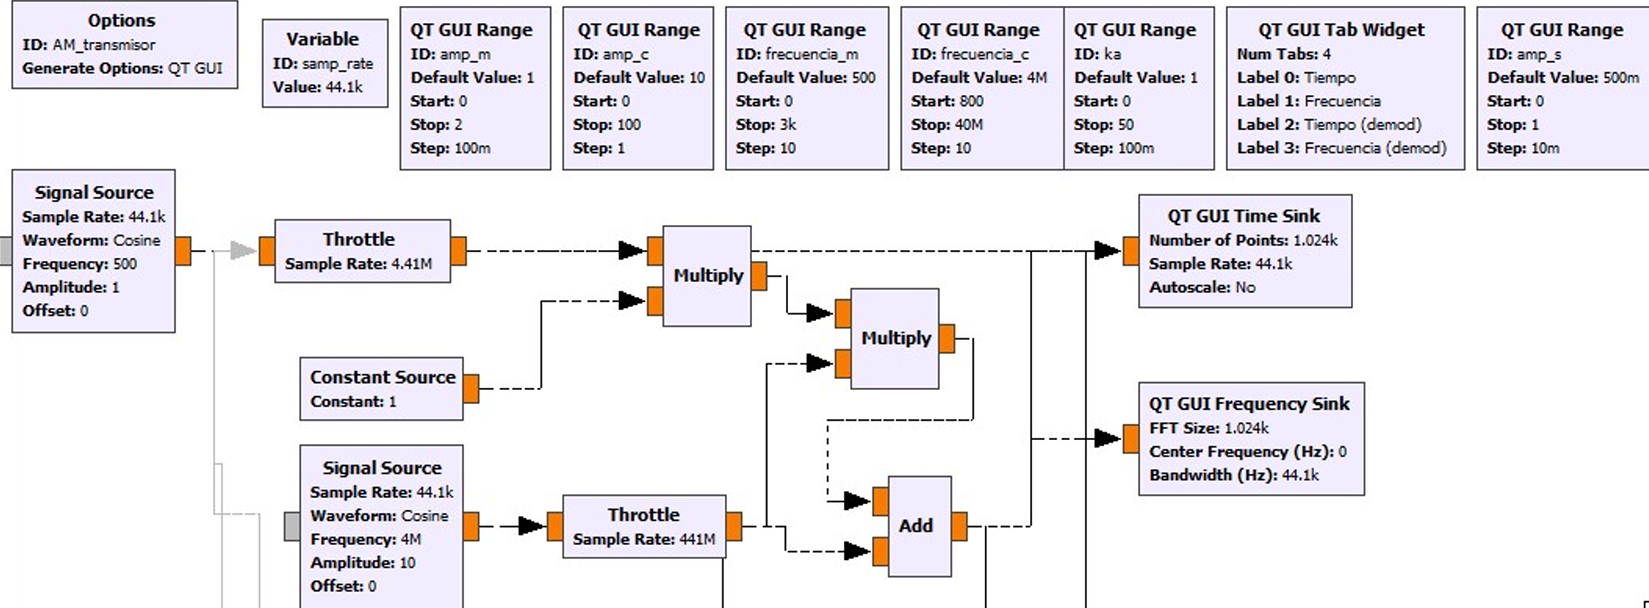
\includegraphics[width=0.6\textwidth]{fig3.png}
    \caption{Esquema en GNU Radio}
    \label{fig:3}
\end{figure}

\begin{itemize}
    \item[a)] ¿Qué es GNU Radio?  
    \item[b)] ¿Qué es SDR?  
    \item[c)] Expresar $s(t)$.  
    \item[d)] Explicar bloques de la Fig.~\ref{fig:3}.  
    \item[e)] Graficar señales para 10\%, 60\% y 100\%.  
    \item[f)] Graficar sobre-modulación.  
    \item[g)] Analizar espectro en cada caso.  
    \item[h)] Implementar receptor y recuperar señal.  
\end{itemize}
	\section{Ejercicio 7}

Diseñar en GNU Radio un modulador que genere una señal de Doble Banda Lateral con Portadora Suprimida. Indicar cuál es la diferencia de espectro con la señal del ejercicio anterior.


    \section{Actividad 8}

Determinar frecuencia instantánea de:  

\[
x_1(t)=2\cos(20\pi t + \phi), \quad
x_2(t)=17\cos(30\pi t + 4\cos(2\pi t)), \quad
x_3(t)=\cos(25\pi t)\cos(2\cos(7\pi t)) + \sin(25\pi t)\sin(2\cos(7\pi t))
\]  



    \section{Actividad 9}

\subsection*{Si se tiene una señal $s(t) = 15\cos(\omega_c t + 2\cos(\omega_m t))$, donde \( f_m = 6~\text{kHz} \) y \( f_c = 72~\text{MHz} \). Obtener:}

\subsection*{a) Si \( k_p = 20~\text{rad/V} \), dar la expresión matemática para la tensión \( m(t) \) de modulación de fase correspondiente. ¿Cuál es su valor pico de tensión y su frecuencia modulante?}

La expresión general de una señal modulada en PM es:
    \[
        s(t) = A_c \cos(2\pi f_c t + k_p m(t))
    \]

Se obtiene que la señal:
    \[
        s(t) = 15\cos(\omega_c t + 2\cos(\omega_m t))
    \]

donde:
    \[
      \omega_c = 2\pi f_c = 2\pi\times72~[MHz] = 144000000\pi~[\text{rad/s}]
    \]
    \[
        \omega_m = 2\pi f_m = 2\pi \times 6~[kHz] = 12000\pi~[\text{rad/s}]
    \]

Comparando con la forma general:
    \[
        k_p m(t) = 2\cos(12000\pi t)
    \]
    
Despejando la señal de mensaje $m(t)$ se obtiene que:
    
    \[
        m(t) = \frac{2}{k_p}\cos(1200\pi t) = 0.1\cos(12000\pi t)~[\text{V}]
    \]
    \[
        m(t) = 0.1\cos(12000\pi t)~[\text{V}
    \]

Por lo tanto, el valor pico de tensión es $V_p = 0.1~[\text{V}]$ y la frecuencia modulante es $f_m = 6~\text{kHz}$

\subsection*{b) Si $k_f = 5\times10^3~\text{rad/V}$, dar la expresión matemática para la tensión $m(t)$ de modulación de frecuencia correspondiente. ¿Cuál es su valor pico de tensión y su frecuencia modulante?}

La forma general de una señal modulada en FM es:
\[
s(t) = A_c \cos\left(2\pi f_c t + 2\pi k_f \int_0^t m(\tau)\,d\tau \right)
\]

Se tiene la siguiente señal:
    \[
        s(t) = 15\cos(\omega_c t + 2\cos(\omega_m t))
    \]

Comparando la señal anterior con la forma general de una señal modula en PM se obtiene que:
    \[
        2\cos(\omega_m t) = 2\pi k_f \int_0^t m(\tau)\,d\tau
    \]

Despejando \( m(t) \):

    \[
        \int_0^t m(\tau)\,d\tau = \frac{2}{2\pi k_f}\cos(\omega_m t)
    \]

Derivando ambos lados:
    \[
        m(t) = \frac{2}{2\pi k_f}\frac{d}{dt}[\cos(\omega_m t)] = \frac{2}{2\pi k_f}(-\omega_m \sin(\omega_m t))
    \]
    \[
        m(t) = -\frac{2\omega_m}{2\pi k_f}\sin(\omega_m t)
    \]

Sustituyendo valores numéricos se obtiene que la señal del mensaje $m(t)$ es:

    \[
        m(t) = -\frac{2(12000\pi)}{2\pi(5\times10^3~[rad/V])}\sin(12000\pi t)
    \]
    \[
        m(t) = -2.4\sin(1.2\times10^4 t)
    \]

Convirtiendo el seno a coseno se obtiene finalmente que la señal $m(t)$ es:

    \[
        m(t) = 2.4\cos(12000\pi t + 90^\circ)
    \]
    
Por lo tanto, el valor pico de tensión es $V_p = 2.4~[\text{V}]$ y la frecuencia modulante es $f_m = 6~\text{kHz}$

\subsection*{c) Al recibir la señal de tensión $s(t)$ en el receptor, se desarrolla una potencia promedio de $4.5~\text{W}$ en una carga acoplada $R$. Determinar el valor de $R$.}

En un resistor \( R \), la potencia promedio es:
    \[
        P = \frac{1}{2}\frac{A_c^2}{R}
    \]

Despejando \( R \):
    \[
        R = \frac{A_c^2}{2P} = \frac{(15~[\text{V}])^2}{2(4.5~[\text{W}])} = 25~[\Omega]
    \]

    \[
        \boxed{R = 25~[\Omega]}
    \]
    \section{Actividad 10}

Una portadora de 97.3 MHz es modulada en FM por 25 kHz con desviación 200 Hz.  

\begin{itemize}
    \item[a)] Ancho de banda por Carson.  
    \item[b)] Ancho de banda y $\beta$ si se duplica amplitud.  
    \item[c)] Ancho de banda y $\beta$ si se duplica frecuencia.  
    \item[d)] Ancho de banda y $\beta$ si se duplican ambos.  
\end{itemize}
    \section{Actividad 11}

Transmisor FM (Fig.~\ref{fig:4}) con salida 97.9 MHz y desviación 75 kHz.  

\begin{figure}[h!]
    \centering
    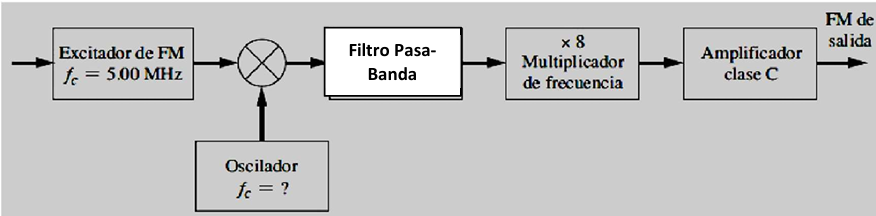
\includegraphics[width=0.6\textwidth]{fig4.png}
    \caption{Diagrama de bloques transmisor FM}
    \label{fig:4}
\end{figure}

\begin{itemize}
    \item[a)] Ancho de banda y frecuencia central del filtro.  
    \item[b)] Frecuencia del oscilador.  
    \item[c)] Capacidad de desviación pico requerida.  
    \item[d)] Índice de modulación.  
    \item[e)] Separación de frecuencias laterales adyacentes.  
\end{itemize}
    \section{Actividad 12}

\subsection*{Se tiene una señal 
$
m_1(t) = A_{m1}\cos(2\pi f_{m1}t)
$
y una señal 
$
m_2(t) = A_{m2}\cos(2\pi f_{m2}t)
$
que se aplican a los canales izquierdo y derecho respectivamente, 
de un generador de señal modulante para FM estéreo.  
Si $m_1(t)$ es de $2~V_{pp}$ y $f_{m1} = 5.2~\text{kHz}$, mientras que 
$m_2(t)$ es de $3~V_{pp}$ y $f_{m2} = 6~\text{kHz}$, graficar la respuesta en frecuencia 
de la señal $m(t)$ que modulará a una portadora de $101.7~\text{MHz}$ 
de un transmisor de FM estéreo.}


Se tienen las siguientes señales:

\begin{itemize}
    \item $m_1(t) = cos(2\pi 5200t)$
    \item $m_2(t) = 1.5cos(2\pi 6000t)$
\end{itemize}

La señal multiplexada esta dada por:
    \[
        m(t) = [m_1(t) + m_2(t)] + [m_1(t) - m_2(t)] \cos(4 \pi f_c t) + k\cos(2 \pi f_c t) 
    \]
donde $f_c=19~[kHz]$ y K es la amplitud del tono piloto.\par

Reemplazando los datos en la  señal multiplexada se obtiene:

    \[
        m(t) = [cos(2\pi 5200t) + 1.5cos(2\pi 6000t)] + [cos(2\pi 5200t) 
    \]
    \[
     - 1.5cos(2\pi 6000t)] \cos(4 \pi 190000 t) + k\cos(2 \pi 19000 t) 
    \]
Distribuyendo el $\cos(4 \pi 190000 t)$ se tiene que:
    \[
        m(t) = cos(2\pi 5200t) + 1.5cos(2\pi 6000t) + cos(2\pi 5200t)\cos(4 \pi 190000 t)
    \]
    \[
        - 1.5cos(2\pi 6000t)\cos(4 \pi 190000 t) + k\cos(2 \pi 19000 t) 
    \]
Utilizando la identidad trigonométrica $\cos(\omega_1)\cos(\omega_2) = \frac{1}{2}[\cos(\omega_1 + \omega_2) + \cos(\omega_1 - \omega_2)]$ y que $\cos(4\pi 19000t) = \cos(2\pi 38000t)$, se obtiene que $m(t)$ es:

    \[
        m(t) = \cos(2\pi 5200t) + 1.5\cos(2\pi 6000t) + \frac{1}{2}\cos[2\pi (5200 + 38000)t] 
    \]
    \[
        + \frac{1}{2}\cos[2\pi (5200 - 38000)t] - \frac{1.5}{2}\cos[2\pi (6000 + 38000)t] + \frac{1.5}{2}\cos[2\pi (6000 - 38000)t]
    \]
    \[
         + k\cos(2\pi 19000t)
    \]
    \[
        = \cos(2\pi 5200t) + \frac{3}{2}\cos(2\pi 6000t) + \frac{1}{2}\cos(2\pi 43200t) + \frac{1}{2}\cos(2\pi (-32800)t)
    \]
    \[
        - \frac{3}{4}\cos(2\pi 44000t) - \frac{3}{4}\cos(2\pi (-32000)t) + k\cos(2\pi 19000t)
    \]

Aplicando la transformada de Fourier a la señal $m(t)$ se obtiene que:

    \[
        M(f) = \frac{1}{2}[\delta(f - 5200) + \delta(f + 5200)] + \frac{3}{4}[\delta(f - 6000) + \delta(f + 6000)] 
    \]
    \[
        + \frac{1}{4}[\delta(f - 43200) + \delta(f + 43200)] + \frac{1}{4}[\delta(f - (-32800))
    \]
    \[
         + \delta(f + (-32800))] - \frac{3}{8}[\delta(f - 44000) + \delta(f + 44000)]
    \]
    \[
        - \frac{3}{8}[\delta(f - (-32000)) + \delta(f + (-32000))] 
    \]
    \[
     + \frac{k}{2}[\delta(f - 19000) + \delta(f + 19000)]
    \]

En la Figura \ref{fig:espectro_ej12} se muestra el espectro de la señal m(t).

    \begin{figure}[H]
        \centering
        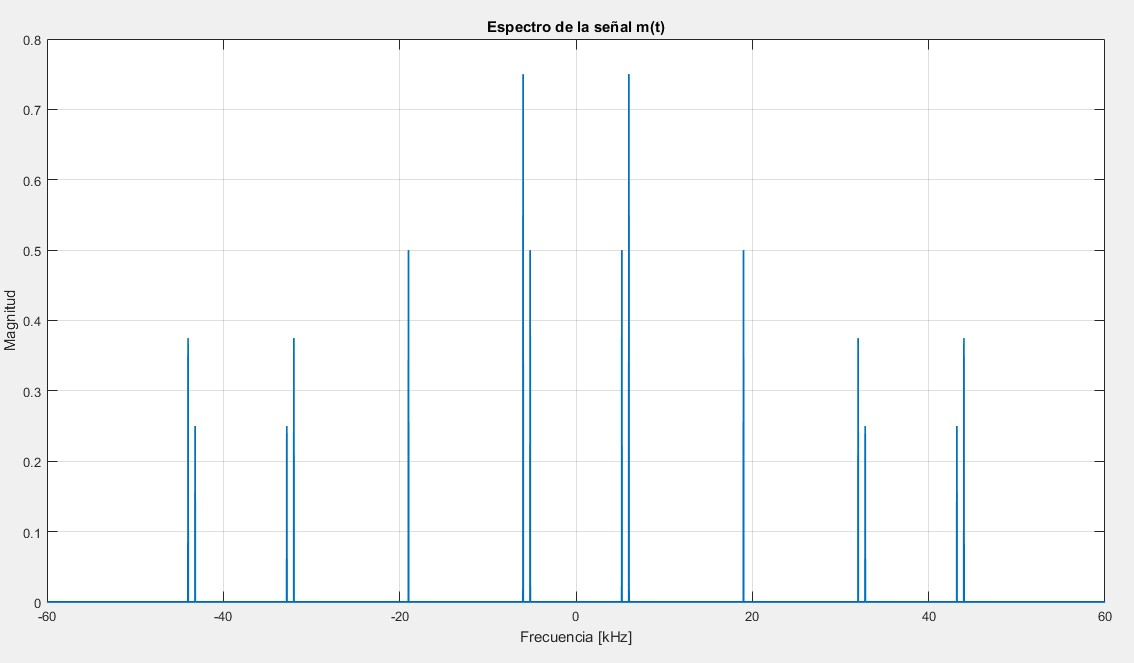
\includegraphics[width=0.8\linewidth]{imagenes/Parte_2/Actividad_12/ejercicio_12.jpg}
        \caption{Espectro de la señal m(t).}
        \label{fig:espectro_ej12}
    \end{figure}
    \section{Actividad 6}

\subsection*{Considerar el diagrama ilustrado en la Fig. \ref{sistema}. Se tiene la primera etapa con un filtro pasa banda, al cual
ingresa ruido blanco Gaussiano, de media cero y densidad espectral de potencia N0/2. Seguido a ello se tiene un modulador producto y 
finalmente un filtro pasa bajo. Las respuestas en frecuencia de ambos filtros pueden observarse en las Fig. \ref{pasabanda} y
Fig. \ref{pasabajo}.}


	\begin{figure}[H]
		\centering
		\includegraphics[width=12cm]{imagenes/Actividad_6/act_6_sistema.jpg}
		\caption{Esquema de la actividad 6.}
		\label{sistema}
	\end{figure}

	\begin{figure}[H]
		\centering
		\includegraphics[width=6cm]{imagenes/Actividad_6/act6_pasabanda.jpg}
		\caption{Respuestas en frecuencia del filtro pasa banda.}
		\label{pasabanda}
	\end{figure}

	\begin{figure}[H]
		\centering
		\includegraphics[width=4cm]{imagenes/Actividad_6/act_6_pbajos.jpg}
		\caption{Respuestas en frecuencia del filtro pasa bajo.}
		\label{pasabajo}
	\end{figure}



\subsection*{a) Calcular la densidad espectral de potencia y la función autocorrelación de $n(t)$. Graficar que se obtiene a la salida 
de cada filtro y del modulador producto (no debe usar el programa).} \par

	La densidad espectral de potencia del ruido $n(t)$ en la salida del filtro pasabanda es:
		\[
			S_{NP_{Banda}}(f) =
			\begin{cases}
			\dfrac{N_0}{2} & -f_c - B < f < -f_c + B \\[6pt]
			\dfrac{N_0}{2} & f_c - B < f < f_c + B \\[6pt]
			0 & \text{o.c.}
			\end{cases}
		\]

	El gráfico de la densidad espectral de potencia a la salida del filtro pasabanda se observa en la Fig. \ref{fig:6pasabanda}.

		\begin{figure}[H]
			\centering
			\includegraphics[width=7cm]{imagenes/Actividad_6/actividad6_pasabanda.jpg}
			\caption{Densidad espectral de potencia del filtro pasabanda.}
			\label{fig:6pasabanda}
		\end{figure}


	Luego, la salida del filtro pasabanda se multiplica por la señal portadora $\cos(2 \pi f_c t)$, donde la transformada de 
	Fourier de dicha portadora es:
		\[
			\cos(2 \pi f_c t) = \tfrac{1}{2} \left[ \delta(f - f_c) + \delta(f + f_c) \right]
		\]
	
	Al multiplicar en el dominio del tiempo, se realiza una convolución en el dominio de la frecuencia, por lo que la densidad espectral de potencia en la 
	salida del modulador producto es:

		\[
			S_{N_{Modulador}}(f) =
			\begin{cases}
			\dfrac{N_0}{4} & -2f_c - B < f < -2f_c + B \\[6pt]
			\dfrac{N_0}{2} & -B < f < B \\[6pt]
			\dfrac{N_0}{4} & 2f_c - B < f < 2f_c + B \\[6pt]
			0 & \text{o.c.}
			\end{cases}
		\]
	
	El gráfico de la densidad espectral de potencia a la salida del modulador producto se observa en la Fig. \ref{fig:6modulador}.


		\begin{figure}[H]
			\centering
			\includegraphics[width=7cm]{imagenes/Actividad_6/actividad6_modulador.jpg}
			\caption{Densidad espectral salida modulador.}
			\label{fig:6modulador}
		\end{figure}



	Finalmente, la salida del modulador producto ingresa al filtro pasabajo, por lo que la densidad espectral de potencia en 
	la salida del filtro pasabajo es:
		\[
				S_{N_{PasaBajo}}(f) =
				\begin{cases}
				\dfrac{N_0}{2} & -B < f < B \\[6pt]
				0 & \text{o.c.}
				\end{cases}
		\]

	El gráfico de la densidad espectral de potencia a la salida del filtro pasabajo se observa en la Fig. \ref{fig:6pasabajo}.
    
		\begin{figure}[H]
			\centering
			\includegraphics[width=7cm]{imagenes/Actividad_6/actividad6_pasabajo.jpg}
			\caption{Densidad espectral salida filtro pasa bajo.}
			\label{fig:6pasabajo}
		\end{figure}

	La función de autocorrelación se obtiene a partir de la transformada inversa de la densidad espectral de potencia, es 
	decir:
		\[
			R_{n(t)}(\tau) = \int_{-\infty}^{\infty} S_{N_{PasaBajo}}(f) e^{j 2 \pi f \tau} df
		\]
	Reemplazando la densidad espectral de potencia obtenida en la salida del filtro pasabajo, se tiene:
		\[
			R_{n(t)}(\tau) = \int_{-B}^{B} \dfrac{N_0}{2} e^{j 2 \pi f \tau} df
		\]
	Resolviendo la integral se obtiene:
		\[
			R_{n(t)}(\tau) = N_0 B \, \text{sinc}(2 B \tau)
		\]
	

\subsection*{b) Calcular la media y la varianza de n(t).} \par

	El ruido blanco gaussiano de entrada tiene media cero, y los filtros lineales e invariantes en el tiempo (filtro pasa banda 
	y filtro pasa bajo) no alteran la media si la entrada tiene media cero. Esto se deduce de la siguiene ecuación:
	
		\[
			\mu_Y = \mu_X \int_{-\infty}^{\infty} h(\tau_1)\, d\tau_1 = \mu_X H(0)
		\]

	Por lo tanto, como la media $\mu_x$ dell ruido en la entrada es cero , entonces la media de $n(t)$ es:
		\[
			\mu_{n(t)} = \mu_x H(0) = 0 \cdot 1 = 0
		\]
	
	Para calcular la varianza se utiliza la siguiente ecuación:

		\[
		\sigma_x^2 = E[x^2] - \mu_x^2
		\]

	Por propiedad de autocorrelación se tiene que \(R_x(0) = E[x^2]\), reemplazando se obtiene lo siguiente:

		\[
		\sigma_x^2 = R_x(0) - 0 = N_0 B \, \text{sinc}(0)
		\]

		\[
		\sigma_x^2 = N_0 B
		\]


\subsection*{c) ¿Cuál es la tasa a la cual $n(t)$ puede ser muestreada, de manera tal de que las muestras resultantes sean no
 correlacionadas?} \par

	Para que las muestras resultantes sean no correlacionadas se busca que la función de autocorrelación sea igual a 0. Entonces,
	teniendo en cuenta la Ecuación 8, esta función da 0 cuando el valor dentro del seno cardinal es un entero
		

		\[
			2B\tau = k, \quad k \in \mathbb{Z}
		\]

	Entonces

		\[
			\tau = \frac{k}{2B}
		\]

		\[
			f_{\text{muestreo}} = \frac{2B}{k}
		\]

	Por lo tanto, la tasa de \(n(t)\) debe ser al menos \(2B\) muestras por segundo para que las muestras 
	resultantes sean no correlacionadas.

    \section{Actividad 14}

\begin{itemize}
    \item[a)] Abrir y ejecutar \texttt{Modulador\_FM.grc}, analizar número de frecuencias laterales significativas para distintos $\beta$.  
    \item[b)] Ejecutar \texttt{FM\_Comercial.grc}, analizar espectro FM comercial.  
    \item[c)] En grupos, probar archivos \texttt{FM\_Receptor.grc} y \texttt{FM\_Transmisor.grc}, sintonizar SDRs y analizar espectros.  
\end{itemize}
    

    

%\printbibliography[heading=bibintoc] % Agrega el título "Referencias" al índice automáticamente
    
\end{document}
